\documentclass[conference]{IEEEtran}

\usepackage{blindtext, graphicx, todonotes, verbatim, url, amsmath, amssymb, subfigure, balance}
% \usepackage{algorithm}
% \usepackage{algpseudocode}
\usepackage{paralist}
\usepackage{amsthm, framed, graphics}
\usepackage{fancybox,fancyvrb}
\usepackage{cite}
\usepackage[
    n,
    advantage,
    operators,
    sets,
    adversary,
    landau,
    probability,
    notions,
    logic,
    ff,
    mm,
    primitives,
    events,
    complexity,
    asymptotics,
    keys]{cryptocode}

% Add the compsoc option for Computer Society conferences.
%
% If IEEEtran.cls has not been installed into the LaTeX system files,
% manually specify the path to it like:
% \documentclass[conference]{../sty/IEEEtran}

% *** GRAPHICS RELATED PACKAGES ***
%
\ifCLASSINFOpdf
  % \usepackage[pdftex]{graphicx}
  % declare the path(s) where your graphic files are
  % \graphicspath{{../pdf/}{../jpeg/}}
  % and their extensions so you won't have to specify these with
  % every instance of \includegraphics
  % \DeclareGraphicsExtensions{.pdf,.jpeg,.png}
\else
  % or other class option (dvipsone, dvipdf, if not using dvips). graphicx
  % will default to the driver specified in the system graphics.cfg if no
  % driver is specified.
  % \usepackage[dvips]{graphicx}
  % declare the path(s) where your graphic files are
  % \graphicspath{{../eps/}}
  % and their extensions so you won't have to specify these with
  % every instance of \includegraphics
  % \DeclareGraphicsExtensions{.eps}
\fi
%

\hyphenation{op-tical net-works semi-conduc-tor}

\newtheorem{definition}{\textbf{Definition}}[section]
\newtheorem{theorem}{\textbf{Claim}}[section]
\newtheorem{corollary}{\textbf{Corollary}}[theorem]
\newtheorem{lemma}[theorem]{\textbf{Lemma}}

\begin{document}

\title{Lightweight Authentication and Access Control for Content-Centric Networks} 

\author{
\IEEEauthorblockN{Ivan O. Nunes and Gene Tsudik}
\IEEEauthorblockA{University of California Irvine \\
\{ivanoliv, gene.tsudik, woodc1\}@uci.edu}
}

\maketitle

\begin{abstract}



\end{abstract}

\begin{IEEEkeywords}
Content-Centric Networking
\end{IEEEkeywords}

\IEEEpeerreviewmaketitle

\section{Introduction}

\nocite{adams1995hitchhiker}

Ideas:
\begin{enumerate}
  \item \emph{krb-ccn} decouples authentication from access control because access rights
	are not associated with the possession of a key not to the ability of decrypting a
	the content's ciphertext (as in attribute-based encryption). Therefore, access control
	policies can be changed without the need to proactively re-distribute access keys.
  \item Users's privacy is preserved since the actual content producers are not aware of which
	is requesting a given content. This is possible because authentication and AC is handled
	by the KDC and not by the final content producer and because of the lack of source addresses
	on CCN interests.
  \item By leveraging the sinenergy between network names in CCN and Kerberos service-names-based AC, we are
	able to provide an effective AC policy by granting AC rights to namespaces (e.g., \emph{/uci/edu/filesystem/userA/*}).
	In IP Kerberos such AC policies are bounded to principals, with are basically names to services within an organization.
	Since in CCN all content is named by design, \emph{krb-ccn} eliminates the need for principals, leading to a cleaner and
	straightforward authentication and authorization system.
  \item \emph{krb-ccn} is also designed with efficiency in mind. As in IP Kerberos, the majority of cryptografic operations in the
	system consist on symmetric-key authenticated encryption. By avoiding computatially expensive operations (sucha as ABC, PKC, and Pairing Based Cryptography),
	\emph{krb-ccn} becomes suitable for scenarios where content producers are resource constrained devices, such as in an evetual CCN-IoT.
  \item The consumer application does not have to be aware of \emph{krb-ccn}. Based on the interest hierarchical name structure,
	the \emph{krb-ccn} local client is capable of fetching the apropriate TGS/TGT, or issue TGS and TGT requests as needed.
\end{enumerate}


Content-Centric Networking (CCN) is an emerging paradigm that emphasizes the transfer
of named data instead of hosts and interfaces. This shifts the security focus from
channels a la protocols such as TLS to the content itself. If content is sensitive
and must be protected, the architecture demands that it be properly encrypted so
that unauthorized consumers cannot view the data. Access control in CCN has been
well studied in recent years. The majority of solutions rely on long-lived public
and private key pairs to protect data. Specifically, data owners or producers
encrypt data under some access control policy with a public key corresponding to
an authorized consumer (or set of consumers). The recipient(s) use their
corresponding private key to decrypt the content.

In principle, this design achieves its goal of providing access control to content.
However, it suffers in two critical problems. The first is revocation. There is an
intrinsic time-of-check versus time-of-use problem with the standard CCN access
control strategy. Specifically, once content is encrypted under a recipient’s
public key, said recipient will always have access to the data barring destruction
of the private key. If a consumer’s access control rights change after content
is published, then said consumer can continue reading the data so long as it can
obtain an encrypted copy. Addressing this problem requires that access to content
always be preceded by an \emph{online} authorization check. Specifically, before
consumer $Cr_i$ accesses content $C(N)$ with name $N$, it must first acquire access
to $C(N)$. Such access will allow $Cr_i$ to read $C(N)$. Moreover, since access to
$C(N)$ at time $t$ might be allowed for $Cr_i$ but not $Cr_j \not= Cr_i$, $C(N)$ must
only be accessible by $Cr_i$. Generalizing this further means that each content is
uniquely encrypted, on demand, for each consumer at time $t$. Thus, encrypted content
must be bound to the state of an access control policy. Otherwise, caching this
content is, in theory, not possible.

The second critical problem is the inadvertent mixing of authentication and authorization.
In the standard approach, there is not online authentication or authorization. Possession
of a private key sufficiently satisfies both purposes. It is up to the producer to
statically enforce its authorization rules by only encrypting content for particular
consumers. This mixture of authentication and authorization is problematic for several
reasons. Firstly, it binds authorization rules to authentication identities. In
applications where authorization checks depend on more than a client identity, this is
not sufficient. Secondly, it requires that authentication be done solely by consumer-owned
private keys. In fact there are many circumstances where a client’s identity is ascertained
using information that is not a private key — passwords being the more prominent counter
example. In summation, it is advantageous to decouple authentication and authorization,
even in CCN. Kerberos is one system that allows us to partly address both of these open
problems. Specifically, Kerberos decouples authentication and authorization services
through the usage of tickets. It also allows services, e.g., content repositories, to
be accessed over an ephemeral session. Tickets permit the service to check the liveness
of authentication information and, therefore, limit the window of data use beyond revocation.

In this paper, we present Hydra, a system inspired by Kerberos for online access control
enforcement in CCN. Hydra separates consumer authentication and authorization into
separate services. It uses tickets or cookies to allow consumers to convey authorization
permissions to target servers, e.g., content repositories. Servers can use these cookies
to determine if requested content should be provided or not. Hydra also introduces a
novel naming scheme to bind consumer credentials to protected content objects. This
allows only authorized consumers to derive the names of protected content objects.
Producers use these derived names when checking authorization rights for target content
or namespaces. This naming scheme is orthogonal to Hydra and may be used in other
application settings to better make access control decisions.

\section{Access Control Restrictions}

CCN supports two types of content restrictions: {\tt KeyIdRestriction}
and {\tt ContentObjectHashRestriction}, or KeyID and ContentID, respectively.
The KeyID restricts content to that which is signed by a key whose hash matches
the KeyID. The ContentID restricts content to that which hashes to the ContentID.
Each of these restrictions can be used by any entity in the network, especially
routers, to verify content.

In this section, we advocate for a new restriction called an {\tt AccessRestriction},
or AccessID. The AccessID is designed to restrict content to that which satisfies
a given access control policy. An access control policy is one which binds a given
content to a specific decryption key. As such, only the owner of the decryption
can generate an AccessID. (This is necessary since, as we will show, AccessIDs serve
as committments to a requests. It must not be possible for a malicious user to forge
a committment to a request.) However, unlike the two prior restrictions, the AccessID
need not be verifiable by any entity in in the network. Confidentiality is an
end-to-end goal and not a feature provided by the network.

Given the obvious asymmetry in roles, this implies the use of a digital signatures
as the AccessID. For example, let $pk$ and $sk$ be public and private key pairs associated with
some access control policy and owned by consumer $Cr$. One trivial construction for AccessID
of $N$ with KeyID $k_ID$ is as follows:
$$
\mathsf{Sign}_{sk}(N || k_ID) || pk
$$
This would bind AccessID to $N$ and the producer's public key. Moreover, it would
allow any network entity to verify this restriction. However, in many cases, this
is overly revealing. Routers need not concern themselves with whether or not a
content matches the requested AccessID. A better construction would therefore limit
exposing this information to the network. Consider the following alternative:
$$
\mathsf{Sign}_{sk}(N || pk || k_ID) || H(N || pk || k_ID)
$$
This restricts verificaftion of the AccessID to those who know $pk$, which is not
otherwise revealed to the network.

An AccessID is inspired by the work of Ghali et al. \cite{ibac15} on
\emph{interest-based access control}. The idea is to bind principals to
interests and then make coupled authentication and authorization decisions
based on this binding. 

\section{Hydra Design}

\subsection{Namespace Based Authorization}

There are at least two fundamental problems one must address in any access control
system: (1) how access control policies are represented and (2) how they are enforced.
Policy representation specifies how policies are mapped onto resources (or content).
For example, one representation might map content names to sets of public keys. These
keys could be owned by authorized consumers and are used when encrypting content.
Encrypting content with name $N$ under a key $pk$ restricts access to the owner of
the corresponding private key. The challenge is to devise a representation that
scales well with the number of resources (content) and consumers. Regardless of
the approach, we claim there is one fundamental feature that must be present for
every access control decision: consumer requests must be bound to a principal.
This allows the producer or entity serving data to provide the appropriate
representation of the target data to the consumer. To achieve this goal, Hydra
uses AccessIDs described in the previous section.

The second problem is rooted more in system design. Consider what must be done
to satisfy a request for access-controlled content. First, the requestor must
be authenticated to bind the request to a principal. Second, the request must
be authorized to determine if access to the desired content is permissable. Lastly,
the data must be packaged in a protected (encrypted) form for the requestor. Thus,
problem (2) is more about how entities are configured to handle the separate
authentication, authorization, content distribution steps in CCN.

In past work, these roles were often convoluted. In particular, \cite{pre,be}
assumed that the entity which handles data production was also implicitly
responsible for content authentication and authorization. CCN-AC \cite{xx} and
NDN-NBAC \cite{xx} separated the authentication and authorization service from
the data production. Specifically, data owners generate and distribute consumer (principal)
private keys to consumers through out-of-band channels. Data producers receive
the corresponding public keys through a similar channel. These are used to encrypt
randomly generated per-content encryption keys.

Despite this separation, these designs still suffer from the following problems.
{\bf First}, authentication and authorization are unnecessarily coupled, leading
to an inherent ``time of check'' versus ``time of use'' problem. Specifically,
consumers obtain private keys from the data owner at time $t$ and use them to
decrypt content at time $t' > t$. {\bf Second}, if consumers are forced to fetch
their private keys from the data owner, a single point of failure emerges. In
particular, it becomes easy to launch a Denial of Service (DoS) attack on the
data owner by forcing it to perform expensive cryptographic operations, e.g.,
signature verifications.
%% @Ivan, the reasons above are ridiculous -- please add others!

\subsection{Protocol}

Hydra is a system designed to address these problems. It has the following features:
%
\begin{compactitem}
    \item Consumer authentication and content authorization decisions can be separated
    and performed by separate systems in the network. A Hydra administrator can spawn
    any number of authentication endpoints to handle client authentication requests.
    Consumers are unable to fetch data from the authorization agent without having
    first been authenticated.
    \item Authorization decisions are centralized to a single system (or set of synchronized
    systems). This permits each authorization check to be done in real-time without
    introducing any added delay between the subsequent use.
    \item XXX
    \item XXX
    \item XXX
\end{compactitem}
%

\begin{table}
\centering
\caption{Notation summary}
\label{notation}
\begin{tabular}{|l|p{6cm}|}
\hline
Notation    			&  Description  							\\ \hline \hline
$I.name$			&  Name of the issued interest I					\\&\\
$N$				&  A namespace prefix (e.g., /uci/ics/ivan/\*) 				\\&\\
$TGT\_Name$			&  Ticket-granting-ticket name (e.g., /uci/ics/TGT) that will be routed towards authenticator \\&\\
$TGS\_Name$			&  Ticket-granting-service name (e.g., /uci/ics/TGS) that will be routed towards authorizer   \\&\\
$sk_C$      			&  Consumer Secret Key						        \\&\\
$pk_C$			        &  Consumer Public Key, including public UID and certificate        	\\&\\
$k_A$ 	   		 	&  Long term symmetric key shared between Authenticator and Authorizer  \\&\\
$k_P$ 	   		 	&  Long term symmetric key shared between Authenticator and Producer    \\&\\
$s \sample \{0,1\}^{\lambda}$	&  Random ${\lambda}$-bits number generation    	     		\\&\\
$ct = Enc_{k}(pt) $		&  Authenticated Encryption of $pt$ using symmetric key $k$		\\&\\
$pt = Dec_{k}(ct) $		&  Decryption of $ct$ using symmetric key $k$    	     		\\&\\
$ct = Enc_{pk}(pt) $		&  Authenticated Encryption of $pt$ using public key $pk$ 		\\&\\
$pt = Dec_{sk}(ct) $		&  Decryption of $ct$ using secret key $sk$    	     			\\&\\
$\sigma = Sign_{sk}(m) $	&  Signature on message $m$ using secret key $sk$ 			\\&\\
$Verif_{pk}(\sigma,m) $		&  Signature verification using public key $pk$     			\\&\\
\hline
\end{tabular}
\end{table}

\begin{figure}
\begin{center}
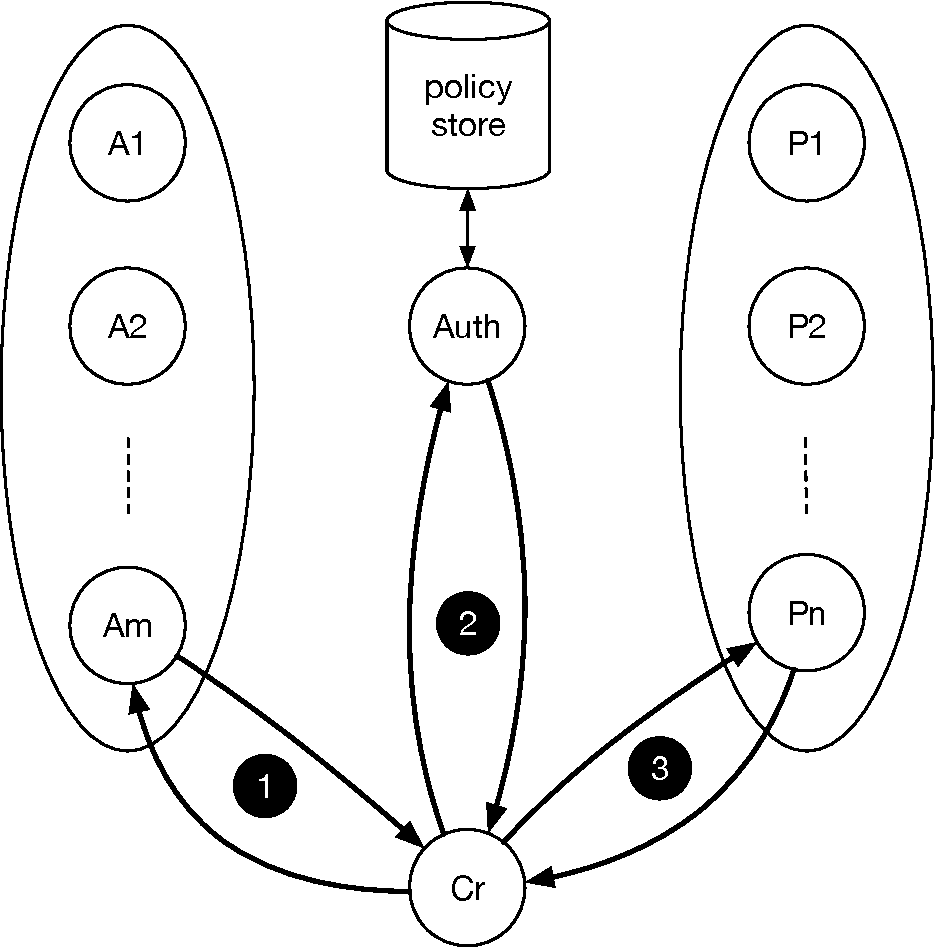
\includegraphics[width=\columnwidth]{Figures/hydra.pdf}
\caption{Hydra system design}
\label{fig:spectr-basic}
\end{center}
\end{figure}




\begin{figure*}
\begin{center}
\fbox{
\procedure{}{%
\textbf{Consumer} \> \> \textbf{Authenticator} \\
\mathsf{I.name = TGT\_Name} \> \> \\
\sigma \gets \mathsf{Sign}_{sk_C}(\mathsf{userName}) \> \> \\
\> \xrightarrow{payload = \sigma, userName} \> \\
\> \> \text{Fetch $pk_C$ according to userName} \\
\> \> \mathsf{Verify}_{pk_C}(\sigma,\mathsf{userName}) \\
%\> \> s \sample \{0,1\}^{\lambda} \\
\> \> t_1 \gets \mathsf{setTGTExpiration}() \\
\> \> k_{TGS} \sample \{0,1\}^{\lambda} \\
\> \> \mathsf{token}_{TGS}^{C} \gets \mathsf{Enc}_{pk_C}(k_{TGS}||t_1) \\
\> \> \mathsf{TGT} \gets \mathsf{Enc}_{k_{A}}(\mathsf{userName} || t_1 || k_{TGS}) \\
\> \xleftarrow{payload = \mathsf{TGT}, \mathsf{token}_{TGS}^{C}} \> \\
k_{TGS}||t_1 \gets \mathsf{Dec}_{sk_C}(\mathsf{token}_{TGS}^{C}) \> \> \\
\mathsf{store(TGT,t_1,k_{TGS})} \> \> \\
}
}
\caption{Consumer authentication protocol}
\label{fig:spectr-basic}
\end{center}
\end{figure*}




\begin{figure*}
\begin{center}
\fbox{
\procedure{}{%
\textbf{Consumer} \> \> \textbf{Authorizer} \\
\mathsf{I.name = TGS\_Name} \> \> \\
\> \xrightarrow{payload=N, \mathsf{TGT}} \> \\
\> \> \mathsf{userName} || t_1 || k_{TGS} \gets \mathsf{Dec}_{k_{A}}(TGT) \\
%\> \> \text{Verify: $s = s'$} \\
\> \> \text{Verify: $t_1$ not expired} \\
\> \> {k_P} \gets \mathsf{verifyPolicyAndFetchKey}(N, \mathsf{userName}) \\ %Kp can be different things (shared key between all boxes that implement that producer, broadcast encryption key, etc)
\> \> k_{N} \sample \{0,1\}^{\lambda} \\
%\> \> r \sample \{0,1\}^{\lambda} \\ why?
\> \> t_2 \gets \mathsf{setTGSExpiration}() \\ %% timestamp
\> \> \mathsf{TGS} \gets \mathsf{Enc}_{k_P}( N || k_N || t_2) \\ %% encrypt the key in the ticket
\> \> \mathsf{token}_N^{C} \gets \mathsf{Enc}_{k_{TGS}}(k_N||t_2) \\
\> \xleftarrow{payload= \mathsf{TGS}, \mathsf{token}_N^{C}} \> \\
k_N || t_2 \gets \mathsf{Dec}_{k_{TGS}}(\mathsf{token}_N^{C}) \> \\
\mathsf{store(N,TGS,t_2,k_N)} \>
}
}
\caption{Consumer-data authorization protocol}
\label{fig:spectr-basic}
\end{center}
\end{figure*}

\begin{figure}
\begin{center}
\fbox{
\procedure{}{%
\textbf{Consumer} \> \> \textbf{Producer} \\
\mathsf{I.name = N||suffix} \> \> \\
\> \xrightarrow{payload= TGS} \> \\
\> \>  N' || k_N || t_2 \gets \mathsf{Dec}_{k_P}(TGS) \\
\> \> \text{Verify: $N'$ is prefix of I.name} \\
%%\> \> \text{Verify: $pk_C'$ = $pk_C$} \\ Not sure this is necessary
\> \> \text{Verify $t_2$ expiration} \\
\> \> D \gets \mathsf{ProduceData}(\mathsf{I.name}) \\
\> \> D' \gets \mathsf{Enc}_{k_N}(D) \\
\> \xleftarrow{payload=D'} \> \\
D \gets \mathsf{Dec}_{K_N}(\mathsf{D'}) \> \> \\
}
}
\caption{Authorization verification protocol}
\label{fig:spectr-basic}
\end{center}
\end{figure}

\begin{figure}
\begin{center}
\fbox{
\procedure{}{%
\textbf{Consumer} \> \> \textbf{Producer} \\
\mathsf{I.name = N||suffix} \> \> \\
\> \xrightarrow{payload= TGS} \> \\
\> \>  N' || k_N || t_2 \gets \mathsf{Dec}_{k_P}(TGS) \\
\> \> \text{Verify: $N'$ is prefix of I.name} \\
%%\> \> \text{Verify: $pk_C'$ = $pk_C$} \\ Not sure this is necessary
\> \> \text{Verify $t_2$ expiration} \\
\> \> D \gets \mathsf{ProduceData}(\mathsf{I.name}) \\
\> \> D' \gets \mathsf{Enc}_{k_N}(D) \\
\> \xleftarrow{payload=D'} \> \\
D \gets \mathsf{Dec}_{K_N}(\mathsf{D'}) \> \> \\
}
}
\caption{Authorization verification protocol including challenge-based consumer authentication}
\label{fig:spectr-basic}
\end{center}
\end{figure}


\subsection{Ivan: Comments}
\begin{enumerate}
 \item IMO, the authentication algorithm (Fig.2) should be unrelated to the namespace you want to get access to. Only related to Consumer's claimed Identity. Otherwise the consumer has to go back to the Authenticator every time she wants a different content (3 RTT).
 \item Unless we are assuming that there is some magical non-deterministic router that will route the same name through different paths, I.name must specify the content produced by the Authenticator, i.e., the TGT. The same applies for TGS.
 \item The TGT as a MAC never expires. My suggestion is to encrypt a timestamp, as in Kerberos, and as we are doing in the authorizer. MAC with an epoch is also an option, but not a good one.
 \item PKE of $K_N$ in the authorization algorithm (Fig 3) could (and maybe should) be symmetric AEAD.
 \item $verifyPolicyAndFetchKey()$ : Could be implemented as broadcast encryption...
 \item Consumer has to receive the expiration date of TGT/TGS. This way Consumer can get back to Authenticator/Authorizer directly, without issuing expired TGT/TGS messages to authorizer/producers.
\end{enumerate}

\section{Conclusions and Future Work}\label{sec:conclusion}
Stuff here, crap there.

\ifCLASSOPTIONcaptionsoff
  \newpage
\fi

\tiny

%\bibliographystyle{IEEEtran}
%\bibliography{hydra}

%\begin{IEEEbiography}[{\includegraphics[width=1in,height=1.25in,clip,keepaspectratio]{picture}}]{John Doe}
%\blindtext
%\end{IEEEbiography}

\end{document}

